%!TEX root = ../../../main.tex

\subsection{Context}

FARO Technologies\textsuperscript{\textregistered} (the parent company of Antares Lda.), is a market leader in the 3D metrology market, with \SI{159.847}[\$]{M} gross profit in 2020 \parencite{faro_2021_financial_results} and a \SI{1.567}[\$]{B} market capitalization as of March 5th, 2021 \parencite{faro_stock_info}. It produces a large variety of devices (from contact and non-contact measurement arms to laser scanners) and a suite of software solutions to integrate FARO's devices into any customer's workflow (CAM2\textsuperscript{\textregistered} and others) \parencite{faro_homepage}.

\begin{figure}[h]
\centering
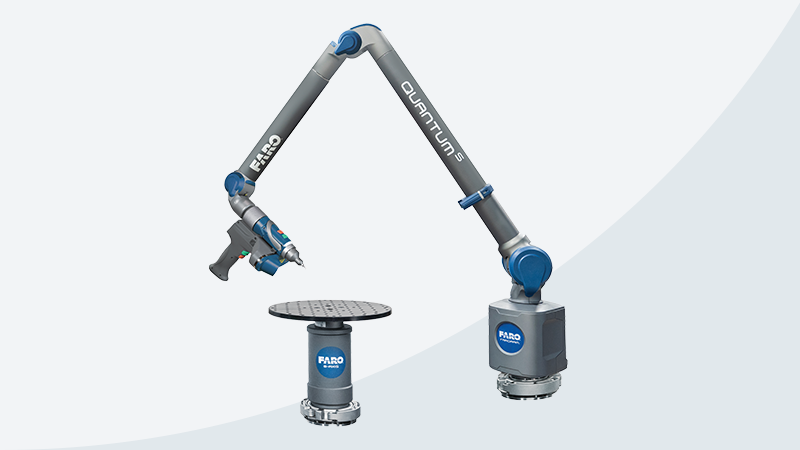
\includegraphics[width=0.7\textwidth]{images/faro_quantum_s_arm.png}
\caption{\faro 8-Axis QuantumS FaroArm\textsuperscript{\textregistered} V2}
\end{figure}
 
\faro's product offerings allow for customers to produce incredibly large data sets (e.g. point clouds from laser line probes such as FAROBlu\textsuperscript{\textregistered} \parencite{faro_quantums}). These sets are a prime candidate for machine learning to be applied to. As such, \faro is investing on research regarding \acrlong{machinel}, which includes the \acrfull{hpo} step in the training of \acrshort{machinel} algorithms.

I took on this challenge as it focuses on an field of research and development that I find interesting.It also allows me to understand if investing my time (in the form of a Master's Degree) in this field would be rewarding and worthwhile.